\documentclass{article}

\usepackage{amsmath}
\usepackage{amsthm}
\usepackage{amssymb}
\usepackage{float}
\usepackage{graphicx}
\usepackage{subfig}
\usepackage[utf8]{inputenc}
\usepackage[english]{babel}

\newtheorem{theorem}{Theorem}

\title{%
	Machine Learning: Collectives of local decision makers\\
	\large Construction Of A Boundary Hunter
}
\author{Daniel Braithwaite}

\begin{document}

\maketitle

The goal of this project is to create neurons which instead of searching for a global minimum they will choose a specific part of the data to place their hyperplane. Consider the following situation in $\mathbb{R}^2$ where we have data split into two classes and the second class is boxed into a chevron shape. A single perceptron will go and place a horizontal line through the plane however this isn't telling us anything interesting. Perhaps something better to do is to align its self to one of the sides of the chevron, then if we added another "boundary hunter" it could align its self to the other side of the chevron.

\section{Simplified Situation}
Before worrying about this in the general case we aim to get a better understanding of the problem by first trying to solve the case described above. We first make some changes to how we have parameterized our perceptron. We want to find a way which performs the same as a standard perceptron before we start making it into a boundary hunter

\subsection{Point \& Gradient Paramaterisation}
We are trying to optimize a point (x,y) and a gradient. This is an alternative way to paramaterise our line. We are using sum squared error for our loss function and sigmoid as our activation. Each "boundary hunter" (BH) has the following weights vector $W = [m, x_0, y_0]$ and we consider two inputs to our BH, x and y. Our perceptron computes $z = (y - y_0) - m(x - x_0)$ and then outputs $o = f(z) = \frac{1}{1+e^{-z}}$.

\subsubsection{Comparison To Perceptron}
If we use the same set of data to train both our standard perceptron and our modified perceptron we see that our modified doesn't quite perform as well as the standard version. For both models below they where trained for 50000 iterations of the training data.

\begin{figure}[H]
\centering
  \begin{minipage}[b]{0.4\textwidth}
    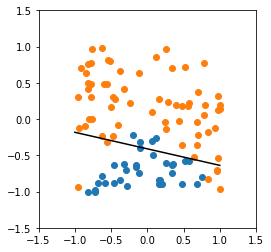
\includegraphics[width=\textwidth]{Standard-Perceptron.png}
    \caption{Standard Perceptron (SSE = 4.90)}
  \end{minipage}
  \hfill
  \begin{minipage}[b]{0.4\textwidth}
    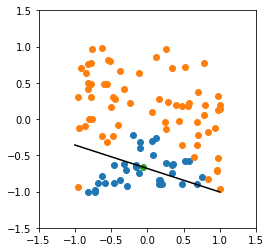
\includegraphics[width=\textwidth]{Modified-Perceptron-(Point-Grad).png}
    \caption{Modified Perceptron (SSE = 7.56)}
  \end{minipage}
\end{figure}

I propose that this way of constructing our perceptron is less powerful than the standard way. Consider when we are optimizing our point-slope representation, 

\begin{align*}
y - y_0 &= m(x - x_0) \\
y &= y_0 + mx - mx_0 \\
y &= mx + (y_0 + mx_0)
\end{align*}

We have just shown that (as we would expect) we can convert out point-slope representation into a intercept-slope representation. From here we see we can convert into something that could be represented by our original perceptron.

\begin{align*}
y = mx + (y_0 + mx_0)\\
\Rightarrow -(y_0 + mx_0) -mx + y
\end{align*}

So given the generic form of our standard perceptron $A + Bx + Cy$ we see here that our modified perceptron can only ever learn a representation where C = 1, limiting what we can achieve. An easy way to check this is to see what happens if we use a standard perceptron to learn the data but keep the third weight (i.e. C) fixed at 1. Sure enough we get the following result when we run that experiment over 50000 iterations.

\begin{figure}[H]
\centering
  \begin{minipage}[b]{0.4\textwidth}
    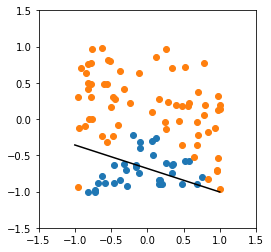
\includegraphics[width=\textwidth]{Standard-Perceptron-(C=1).png}
    \caption{Standard Perceptron with C = 1 (SSE = 7.56)}
  \end{minipage}
  \hfill
\end{figure}

So we are able to conclude that this method is unsuitable

\subsection{Normal \& Point Paramaterisation}
This method involves learning the normal vector (which is what the standard perceptron is doing) along with a point on the hyperplane. This increases the number of parameters we have to learn by n (when we are in $\mathbb{R}^n$ but this is necessary as to implement a BH we have to define some neighborhood in which we care about and to do this we need to define it around some point on our hyperplane. So consider the following situation, we are learning the vector $n = [n_1, ..., n_n]$ normal to our hyperplane, the vector $a = [a_1, ..., a_n]$ which is on our hyperplane. We define $x = [x_1, ..., x_n]$ as our inputs making our weighted sum

\begin{align*}
z = \sum_{i=1}^n n_i * (a_i - x_i)
\end{align*}

We are still using SSE for loss and Sigmoid for activation.

\subsubsection{Comparison To Perceptron}
Like before we compare the two parameterizations using the same data and over 50000 iterations in the 2D case. In the graph for the modified perceptron the green point is our vector on the hyperplane.


\begin{figure}[H]
\centering
  \begin{minipage}[b]{0.4\textwidth}
    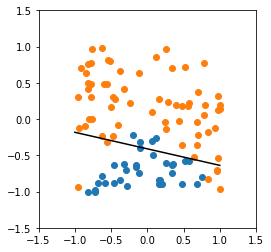
\includegraphics[width=\textwidth]{Standard-Perceptron.png}
    \caption{Standard Perceptron (SSE = 3.90)}
  \end{minipage}
  \hfill
  \begin{minipage}[b]{0.4\textwidth}
    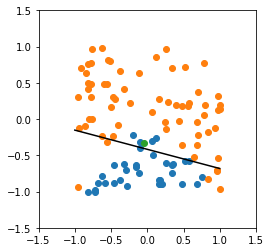
\includegraphics[width=\textwidth]{Modified-Perceptron-(Normal-Point).png}
    \caption{Modified Perceptron (SSE = 3.90)}
  \end{minipage}
\end{figure}

This modified perceptron has all the quality needed to proceed with creating the boundary hunters, whats better is this also generalizes to the $\mathbb{R}^n$ case.

\section{Boundary Hunter}
Using the \textbf{Normal \& Point Parameterization} from before we construct boundary hunters, first we have a simple case where the area of interest for each boundary hunter is simply a circle with fixed radius, our goal is to make this area of interest an ellipse which the BH will learn.

\subsection{Loss Function Design: Attempt 1}
We wish to convert our Perceptron into a Boundary Hunter so to begin we start with designing a suitable loss function. So firstly we want to have some notion of how responsible a boundary hunter is for a given data point, for now we will just denote the responsibility for data point n by $r_n$ and worry about calculating this later. Consider our boundary hunter as reducing the uncertainty of the classes for each of the data points. As the data points get further away from our radius of expertises we become more uncertain about the class of the data point. So a reasonable loss function is 

\begin{align}
\frac{1}{n} \sum_{i=0}^n r_i(C_i log(y_i) + (1-C_i)log(1-y_i)) + (1-r_i) log(1/2)
\end{align}


\subsection{Responsibility Function Design}
How do we construct $r_i$. We would like the following property's of a responsibility function

\begin{enumerate}
\item Making the area of interest include all points will reduce loss to standard log loss.
\item All points inside the area of interest should have the same responsibility.
\item Responsibility for points outside the area of interest should decrease as distance from area increases.
\end{enumerate}

The following function seems like a good place to start. The responsibility for any point inside the area of interest is 1, and as the data points get further away the responsibility decreases

\begin{align}
r_i = 1 - \frac{max(0, d-r)}{abs(d-r) + 0.1}
\end{align}

However we note that this functions isn't smooth, and that can cause problems when training with back prop, not to mention the hard boundary (i.e. responsibility 1 for all points inside area of interest) will also have a negative effect on the gradients. While its reasonable for us to want property (2) it seems unlikely we will find a suitable function meeting the condition. So we remove property (2) and add the condition that our function must be smooth. We now turn to the logistic function, Let $f = 1 - \frac{1}{1 + e^{-S(d - r)}}$, where S is the steepness of the sigmoid. We will want our responsibility function to have a low sensitivity at each extreme, i.e. a small change in distance when the point is either very close to or far from our center point should have a negligible impact on the responsibility. How ever we want our function to be very sensitive around the border of our area of interest. By a purely arbatary decision and from inspecting the graphs I chose to have a steepness of 10 thus giving us the following function

\begin{align}
r_i = 1 - \frac{1}{1 + e^{-10(x-r)}}
\end{align}

While this does not meet our original criteria we see that for most points inside our area of interest the responsibility will be "close" to 1 and certainly above $\frac{1}{2}$, And if the area includes all the points then our loss will not reduce to the standard log loss but it will be close to it and as $r \to\infty$ we will converge to the standard log loss.

\subsubsection{Experimental Results}
We train our boundary hunter over the same data for 10000 iterations and the result is somewhat uninteresting, it simply learns an area of interest which contains no points in the data set

\begin{figure}[H]
\centering
  \begin{minipage}[b]{0.4\textwidth}
    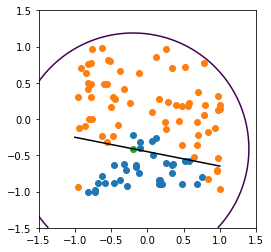
\includegraphics[width=\textwidth]{BoundaryHunter-Attempt1-01.png}
    \caption{Boundary Hunter with (1) as loss and (3) as responsibility}
  \end{minipage}
  \hfill
\end{figure}

As demonstrated using this loss does not produce any significant results.

\subsubsection{Justification For Results}
So consider our loss for a given data point with target $t$, prediction $y$ and responsibility $r$. WILOG assume $t = 1$. So then we are left with $r\ log(y) + (1-r)\ log(\frac{1}{2})$. We know that $log(y) \leq log(\frac{1}{2})$

\subsubsection{Reflection}
Essentially we want to reward our boundary hunter if it is an expert in a given region, so if it gets things wrong outside its area of interest thats good, and if it gets things correct outside its area of interest then thats bad.

\subsection{Loss Function Design: Attempt 2}
Based on our previous findings a more in depth consideration of a suitable loss function is required. Consider the following properties of our ideal loss function. The basic idea is that we want to become experts in a given region
\begin{enumerate}
\item As a data point gets further away from our area of interest we "care less" about our accuracy for classifying that point.
\item Increasing area of interest should decrease the loss iff increasing the area of interest allows us to classify more points correctly.
\item Decreasing area of interest should decrease the loss iff reducing area of interest allows us to classify less points incorrectly in our area
\end{enumerate}

We can simplify these ideas into rules

\begin{enumerate}
\item We want to be as accurate as possible in our area of interest and care less about our accuracy based on how "responsible" we are for the data point.
\item We should be penalized for classifying things correctly out side our area of interest based on how "not responsible" we are for the data point (i.e. if we are classifying a data point correctly but it is just outside our area of interest then we should be penalised).
\item We should be rewarded for classifying things incorrectly our side our area of interest based on how "not responsible" we are for the data point (i.e. if we are classifying a data point incorrectly and its just outside our area of interest then we should be rewarded).
\end{enumerate}

We now wish to convert this into a loss function. Item (1) is referring to $r_n$ multiplied by the standard cross entropy, restricted to points inside our area of interest. Then items (2) + (3) are referring to the opposite of our cross entropy multiplied by $r_n$ restricted to all points outside our area of interest.

\begin{align}
- \big( \frac{1}{|I|} \big[ \sum_{i \in I}^n H(t_i, y_i) \big] + \frac{1}{|O|} \big[ \sum_{i \in O} H(\not t_i, y_i) \big] \big)
\end{align}

Where $I$ is the set of points inside our area and $O$ is the set of points not in our area of interest.

\subsubsection{Experimental Results}

With the same parameters as before we train a perception with this loss and find equally uninteresting results. Essentially the boundary hunter ends up positioning not doing anything useful at all

\begin{figure}[H]
\centering
  \begin{minipage}[b]{0.4\textwidth}
    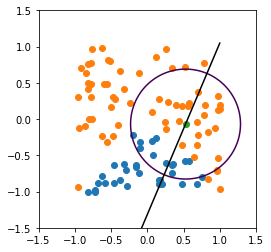
\includegraphics[width=\textwidth]{BoundaryHunter-Attempt2-01.png}
    \caption{Boundary Hunter with (?) as loss and (3) as responsibility}
  \end{minipage}
  \hfill
\end{figure}

\subsubsection{Reflection}
The conditions used to construct this loss are perhaps to harsh, currently we are trying to maximize our error outside while minimizing our error inside. Where we don't actually care how incorrect we are outside our area.

\subsection{Loss Function Design: Important Observation}
We take a step back and consider the basics of what we are trying to achieve. First we make an interesting observation which will change the way we approach designing this loss. Consider the simple loss function $L =\sum R(r) * CE$ where $R(r)$ is our responsibility function with radius as parameter and $CE$ is our cross entropy. And we want to compute the quantity $\frac{\partial r}{\partial L}$ so we can train r. We observe the following

\begin{align*}
\frac{\partial L}{\partial r} &= \frac{\partial}{\partial r} \big[ \sum R(r) * CE \big] \\
&= \sum R^{'} (r) * CE
\end{align*} 

Namely the quantity $\frac{\partial L}{\partial r}$ doesn't actually tell us how changing the radius changes the error it simply tells us which direction to move the radius to increase the responsibility. This results in the radius constantly increasing.\\

\subsection{Loss Function Design: Attempt 3}
Based on what we just observed we need a new approach. We consider our boundary hunter as a sales man, who gets paid $\$B$ for selling something to someone who wants it (if the sales man is responsible for this individual) and gets penalized $\$C$ dollars for selling something to someone who doesn't want it. Using this model, the sales man's is to position them selves and adjust there responsibility so that they are maximizing there profit. Now we simply must quantify this. We know $y^t(1-y)^{t-1}$ is the probability we get something right (probability we are selling to someone who wants what we are selling). We arrive at the flowing quantity.

\begin{align}
L = \sum_{i=0} r_i * \big[Cy_i^{1-t_i}(1-y_i)^{t_i} - By_i^{t_i}(1-y_i)^{1-t_i} \big] 
\end{align}

While initially it seemed like this would suffer from the same problem described in the previous observation it does not. Consider the differential we know that $R^{'}(r)$ will always have the same sign but $Cy_i^{1-t_i}(1-y_i)^{t_i} - By_i^{t_i}(1-y_i)^{1-t_i} $ can be both positive and negative, so we end up in the situation where if we are losing more money that we are gaining then we will decreases our radius but if we are gaining more money than we are losing we will increase our radius

\subsubsection{Experimental Results}

With the same parameters as before we train a perception with this loss and find that it grows to fit all the data

\begin{figure}[H]
\centering
  \begin{minipage}[b]{0.4\textwidth}
    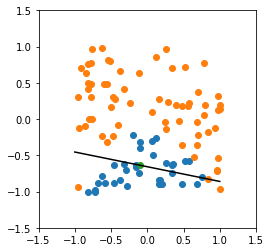
\includegraphics[width=\textwidth]{BoundaryHunter-Attempt3-01.png}
    \caption{Boundary Hunter with (5) as loss and (3) as responsibility}
  \end{minipage}
  \hfill
\end{figure}

Not quite the results we where looking for but this outcome makes sense as there is a disproportionate amount of points. Increasing the parameter C will allow us to tune our boundary hunter to care more about getting things incorrect. To get a good spread we use C = 2, 2.5, 3

\begin{figure}[H]
  \centering
  \begin{minipage}[b]{0.49\textwidth}
    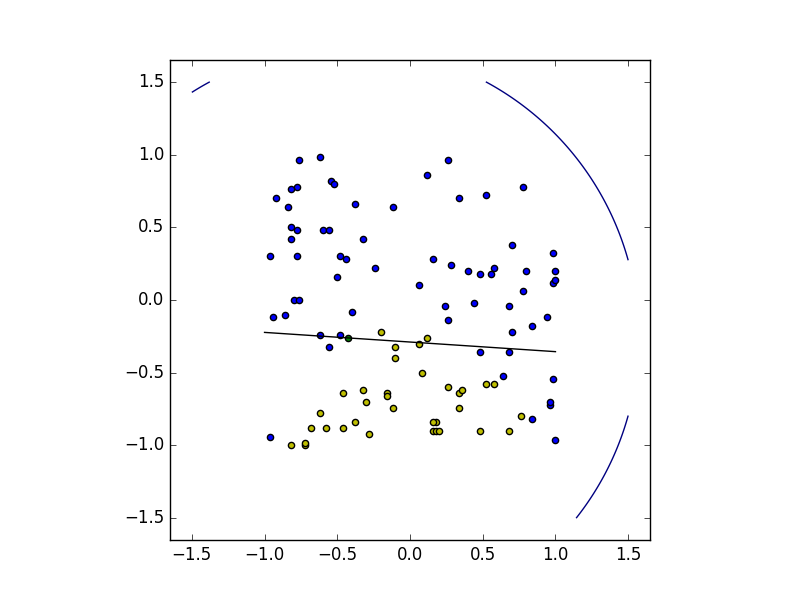
\includegraphics[width=\textwidth]{BoundaryHunter-Attempt3-02.png}
    \caption{C = 1.3}
  \end{minipage}
  \hfill
  \begin{minipage}[b]{0.49\textwidth}
    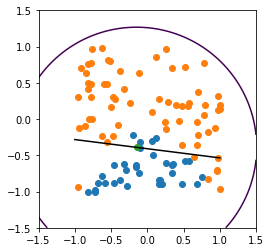
\includegraphics[width=\textwidth]{BoundaryHunter-Attempt3-03.png}
    \caption{C = 1.6}
  \end{minipage}
  \hfill
  \begin{minipage}[b]{0.49\textwidth}
    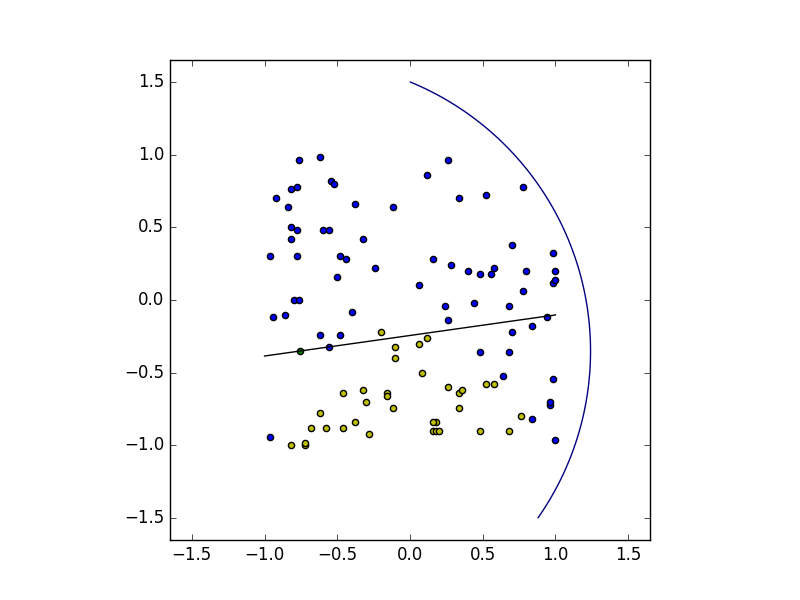
\includegraphics[width=\textwidth]{BoundaryHunter-Attempt3-04.png}
    \caption{C = 1.9}
  \end{minipage}
\end{figure}

How ever this only seems to change the positioning of the hyperplane and not the radius of our area of interest. If we impose some reasonable restrictions on the radius (i.e. $0.3 \leq r \leq 0.8$), set our C = 2 and adjust the responsibility function to be less steep (steepness of 5) then we can achieve some results which seem interesting

\begin{figure}[H]
  \centering
  \begin{minipage}[b]{0.4\textwidth}
    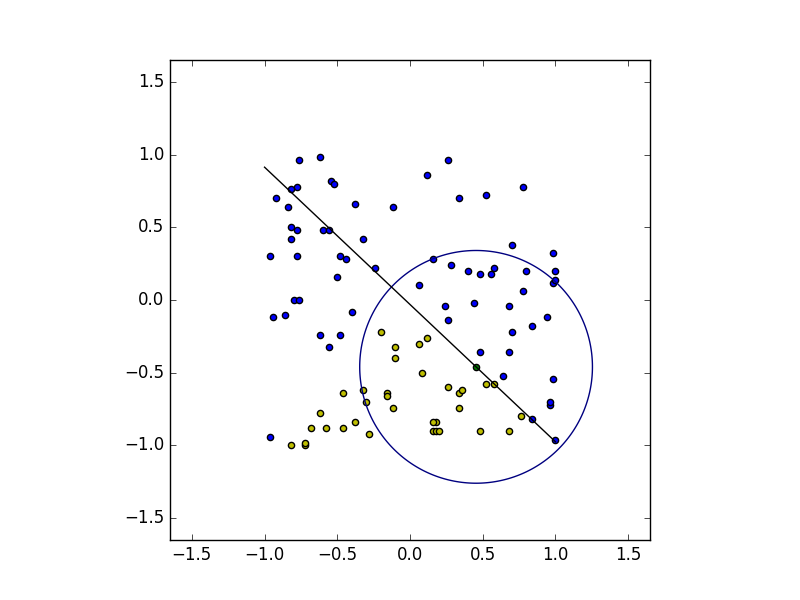
\includegraphics[width=\textwidth]{BoundaryHunter-Attempt3-R0.png}
    \caption{}
  \end{minipage}
  \hfill
  \begin{minipage}[b]{0.4\textwidth}
    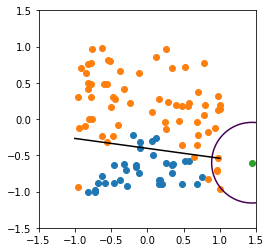
\includegraphics[width=\textwidth]{BoundaryHunter-Attempt3-R1.png}
    \caption{}
  \end{minipage}
  \hfill
\end{figure}

However more often than not we get results like following uninteresting ones

\begin{figure}[H]
  \centering
  \begin{minipage}[b]{0.5\textwidth}
    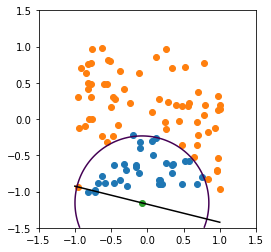
\includegraphics[width=\textwidth]{BoundaryHunter-Attempt3-R2.png}
    \caption{}
  \end{minipage}
  \hfill
\end{figure}

The issue appears to be that of local optima, the solutions looking like what we want (Figure 13 and 14) certainly have lower error than when the solutioin is outside the data however the boundary hunter appears to have trouble escaping local optima to find these more interesting solutions.

To confirm this we look to plot the landscape of the loss function. To do this we will fix the radius and and the hyperplane position while varying the x and y position of the point, The parameters we fix for hyperplane are what we would want if trying to place our self on the left side of the chevron . Using the parameters as above, (steepness of 5, C = 2) We get the following plots.

\begin{figure}[H]
  \centering
  \begin{minipage}[b]{0.8\textwidth}
    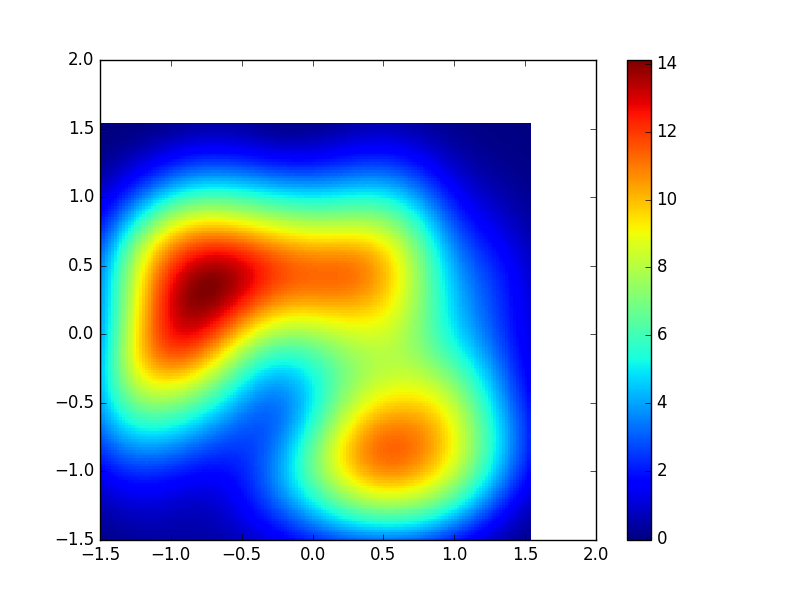
\includegraphics[width=\textwidth]{LossPlot-1.png}
    \caption{Radius as 0.3}
  \end{minipage}
  \hfill
\end{figure}

\begin{figure}[H]
  \centering
  \begin{minipage}[b]{0.8\textwidth}
    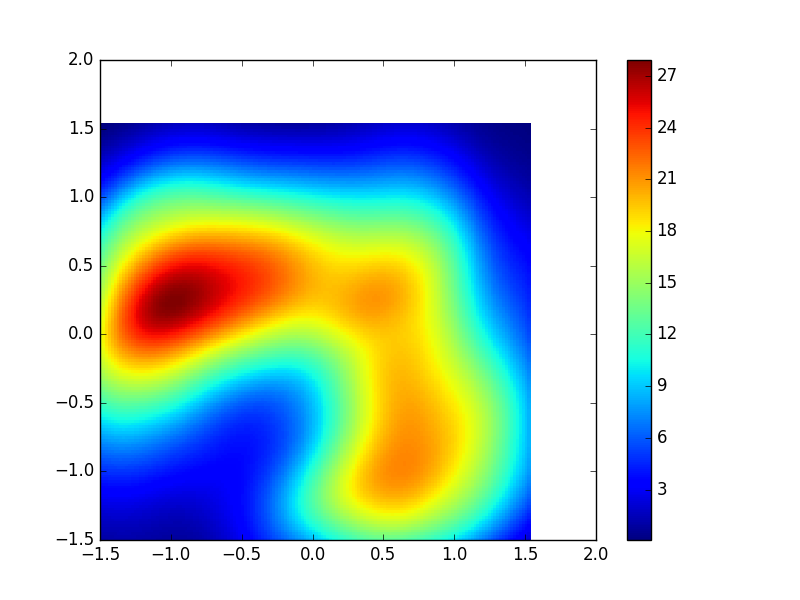
\includegraphics[width=\textwidth]{LossPlot-2.png}
    \caption{Radius as 0.8}
  \end{minipage}
  \hfill
\end{figure}

\begin{figure}[H]
  \centering
  \begin{minipage}[b]{0.8\textwidth}
    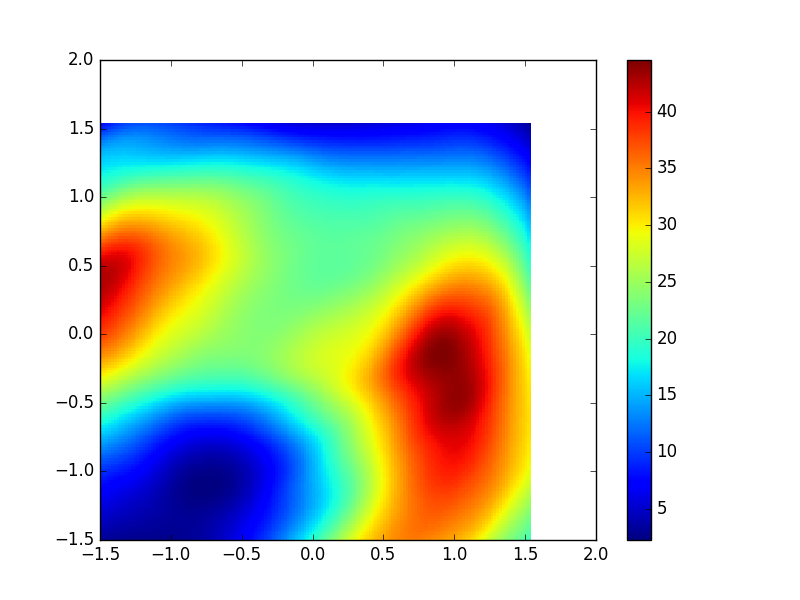
\includegraphics[width=\textwidth]{LossPlot-3.png}
    \caption{Radius as 2.0}
  \end{minipage}
  \hfill
\end{figure}

As clearly demonstrated by these graphs this loss function is not condusive to finding the optimal solution we are expecting.  There is a noticeable deformation in the contour where our expected solution is however it is unlikely that it will be found by the boundary hunter, more often than not we will end up on the outside of the data. For points outside our area of interest the responsibility rapidly approaches 0, this is what would cause the edge of the data to be an optimal solution. While this would indicate a responsibility function which is to steep, adjusting this has little effect.

\begin{figure}[H]
  \centering
  \begin{minipage}[b]{0.8\textwidth}
    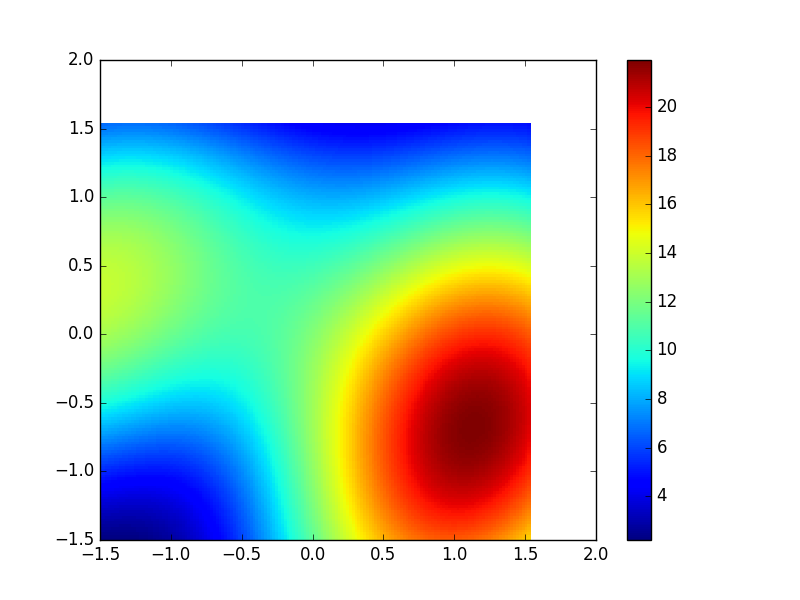
\includegraphics[width=\textwidth]{LossPlot-4.png}
    \caption{Radius as 0.3, with steppness as 0.5}
  \end{minipage}
  \hfill
\end{figure}

\end{document}
